\documentclass[13pt,a4paper]{report}
\usepackage[margin=0.6in]{geometry}
\usepackage{fancybox}
\usepackage[utf8]{inputenc}
\usepackage[vietnamese,main=english]{babel}
\usepackage{multicol}
\usepackage{tabularx}
\usepackage{lmodern}
\usepackage{indentfirst}
\usepackage{float}
\usepackage{enumitem}
\usepackage{afterpage}
\usepackage[super]{nth}
\usepackage{titlesec}
\usepackage{bigdelim}
\usepackage[titles]{tocloft}
\usepackage{makecell}
\usepackage{arydshln}
\usepackage{perpage} %the perpage package
\usepackage{graphicx}
\usepackage{caption}
\usepackage{minted}
\usepackage{gensymb}
\usepackage{tikz}
\usepackage{circuitikz}
\usepackage{pgfplots}
\usepackage{cancel}
\usepackage{xurl}
\usepackage[bottom]{footmisc}
\usepackage[font=footnotesize,labelfont={scriptsize}]{subfig}
\usepackage{wrapfig}
\usepackage{latexsym,amssymb,amsmath}
%\usepackage{algpseudocode}
\usepackage{tocvsec2}
\usepackage{fancyref}
\usepackage{bookmark}
\usepackage{hyperref}
\usepackage[nameinlink,noabbrev]{cleveref}

\newcolumntype{Y}{>{\centering\arraybackslash}X}

\PassOptionsToPackage{hyphens}{url}

\makeatletter
\pgfcircdeclarebipole{}{\ctikzvalof{bipoles/vsourceam/height}}{vsourceAM}{\ctikzvalof{bipoles/vsourceam/height}}{\ctikzvalof{bipoles/vsourceam/width}}{%
  \pgfsetlinewidth{\pgfkeysvalueof{/tikz/circuitikz/bipoles/thickness}\pgfstartlinewidth}
   \pgfpathellipse{\pgfpointorigin}{\pgfpoint{0}{\pgf@circ@res@up}}{\pgfpoint{\pgf@circ@res@left}{0}}
   \pgfusepath{draw}
   \pgfscope
       \pgftransformxshift{0.6*\ctikzvalof{bipoles/vsourceam/margin}\pgf@circ@res@left}
       \pgftext[rotate=-\pgf@circ@direction]{$+$}
       \pgfusepath{draw}
   \endpgfscope
   \pgfscope
       \pgftransformxshift{0.6*\ctikzvalof{bipoles/vsourceam/margin}\pgf@circ@res@right}
       \pgftext[rotate=-\pgf@circ@direction]{$-$}
       \pgfusepath{draw}
   \endpgfscope
}
\makeatother

\MakePerPage{footnote} %the perpage package command
\usetikzlibrary{shapes,positioning,arrows,calc,automata}

\newcommand*\justify{%
  \fontdimen2\font=0.4em% interword space
  \fontdimen3\font=0.2em% interword stretch
  \fontdimen4\font=0.1em% interword shrink
  \fontdimen7\font=0.1em% extra space
  \hyphenchar\font=`\-% allowing hyphenation
}
\renewcommand\cftchapafterpnum{\vskip-2pt}
\renewcommand\cftsecafterpnum{\vskip-2pt}

\renewcommand{\theequation}{\arabic{equation}}

% FLOW CHART
\tikzstyle{startstop} = [rectangle, rounded corners, minimum width=3cm, minimum height=1cm,text centered, draw=black, fill=red!30]
\tikzstyle{io} = [trapezium, trapezium left angle=70, trapezium right angle=110, minimum width=3cm, minimum height=1cm, text centered, draw=black, fill=blue!30]
\tikzstyle{process} = [rectangle, minimum width=3cm, minimum height=1cm, text centered, draw=black, fill=orange!30, text width=4cm]
\tikzstyle{decision} = [diamond, aspect=2.5, minimum width=3cm, minimum height=1cm, text centered, draw=black, fill=green!30]
\tikzstyle{arrow} = [thick,->,>=stealth]

% CHAPTER FORMAT
\titleformat{\chapter}%[display]
{\bfseries\fontsize{25}{30}\selectfont\raggedright}% Format and size of title text
{\llap{%
    \rule[-6pt]{6cm}{1.18cm}\rule{6pt}{0pt}}% Black box to the left, lowered 6pt. The end rule is a horisontal space.
  \llap{% Number also to the left, on top of the black box.
    \fontsize{22}{44}\selectfont\color{white}\thechapter\rule{10pt}{0pt}}}{0pt}{}{}

\counterwithin{figure}{section}
\renewcommand{\thefigure}{\arabic{chapter}.\arabic{section}.\alph{figure}}

\renewcommand{\thetable}{\arabic{table}}

\renewcommand\labelitemi{$-$}
  
\titleformat{\section}
  {\LARGE\bfseries}{}{}{}
\renewcommand\thesection{\arabic{section}.}
\renewcommand\thesubsection{\arabic{subsection}}
\makeatletter
\renewcommand*\l@section{\@dottedtocline{1}{1.5cm}{2em}}
\renewcommand\section{\@startsection {section}{1}{-1em}%
  {-3.5ex \@plus -1ex \@minus -.2ex}%
  {2.3ex \@plus.2ex}%
  {\normalfont\Large\bfseries}}
\def\sectionmark#1{%
      \markright {\MakeUppercase{#1}}}
\makeatother

\titleformat{\subsection}
  {\normalfont\bfseries}{\thesubsection.}{0.5em}{}
\renewcommand\cftsubsecaftersnum{.} 
\renewcommand\thesubsection{\alph{subsection}}

\addto{\captionsenglish}{%
  \renewcommand{\bibname}{References}
}

%\addtocontents{toc}{\setcounter{tocdepth}{2}}
%\addtocontents{lof}{\vskip -1.6cm}
%\addtocontents{lot}{\vskip -1.6cm}

    
% TOC settings
\renewcommand\cftchapnumwidth{2.8em}
\renewcommand\cftsecnumwidth{3em}
\renewcommand\cftsecindent{3em}
\renewcommand\cftsubsecindent{5em}
\renewcommand\thechapter{\Roman{chapter}}
    
%\titleformat{\chapter}[display]{\normalfont\huge\bfseries}{}{0pt}{\Huge}
\newcommand{\hsp}{\hspace{20pt}}
%\titleformat{\chapter}[hang]{\Huge\bfseries}{\thechapter\hsp\textcolor{gray75}{|}\hsp}{0pt}{\Huge\bfseries}
\titleformat*{\subsubsection}{\large\bfseries}
%\titlespacing*{\chapter}{0pt}{0pt}{0pt}
    
\newcolumntype{P}[1]{>{\centering\arraybackslash}p{#1}}
\newcolumntype{C}{>{\centering\arraybackslash}p{4em}}
    
\setlist[itemize]{noitemsep, topsep=0pt}
%\AtBeginEnvironment{multicols}{\RaggedRight}

\titlespacing*{\chapter}{0pt}{0pt}{20pt}

\newcommand\Chapter[2]{\chapter
  [#1\text{: }\hfil\hbox{}\protect\linebreak{\itshape#2}]%
  {#1\\[-0.75ex]\Large#2}%
  \markboth{\MakeUppercase{\chaptername\ \thechapter.\ #1}}{}%
}


\def\doubleoverline#1{\overline{\overline{#1}}}

\captionsetup[subfloat]{labelformat=empty}

\begin{document}
%Trang bìa 1
\fontsize{13pt}{18pt}\selectfont
\begin{titlepage}
\thispagestyle{empty}
\thisfancypage{%đóng khung trang này
\setlength{\fboxsep}{0pt}% 8pt là độ dày của đường viền
\fbox}{} % phần nội dung sau là tương tự như đã làm
\

\begin{center}
\begin{large}
HO CHI MINH CITY UNIVERSITY OF TECHNOLOGY $-$ VNU HCMC
\end{large} \\
\begin{large}
OFFICE FOR INTERNATIONAL STUDY PROGRAM
\end{large} \\
\begin{large}
FACULTY OF ELECTRICAL AND ELECTRONIC ENGINEERING
\end{large} \\
\textbf{--------------------  *  --------------------}\\[4cm]

\includegraphics[scale=0.1]{logobk.png}\\[1cm]
{\fontsize{20pt}{1}\selectfont DIGITAL SYSTEMS (LAB)}\\
{\fontsize{20pt}{1}\selectfont EXPERIMENTAL REPORT (PreLab 5)}\\[2.5cm]
\end{center}

\begin{otherlanguage}{vietnamese}
\begin{tabbing}
	\hspace{3.5cm}Lecturer  \ \ \ \ \=: \textbf{\parbox[t]{9cm}{Mr. Nguyễn Tuấn Hùng}}\\
	\hspace{3.5cm}Subject \>: \textbf{\parbox[t]{12cm}{Digital Systems}}\\
	\hspace{3.5cm}Class \>: \textbf{\parbox[t]{9cm}{TT06}}\\
	\hspace{3.5cm}Name \>: \textbf{\parbox[t]{9cm}{
		Lương Triển Thắng}}\\
	\hspace{3.5cm}Student ID \>: \textbf{\parbox[t]{9cm}{
		2051194}}\\[40pt]
\end{tabbing}
\end{otherlanguage}

\vspace{2.25cm}
\begin{center}
{\fontsize{13pt}{1}\selectfont Ho Chi Minh City, \nth{7} June, 2022}
\end{center}
\end{titlepage}

\tableofcontents

\setminted{fontsize=\normalsize}

\setcounter{chapter}{4}

\Chapter{Pre Laboratory 5}{A simple processor}

\section{Known how to convert instructions to machine codes}
\subsection{Describe the instructions}
\begin{table}[H]
\centering
\begin{tabular}{cc|l}
\multicolumn{2}{c|}{Instruction} & \multicolumn{1}{c}{Explain}           \\ \hline
mv            & R1,R4            & Move value in register R1 to R4       \\
mv            & R3,R2            & Move value in register R3 to R2       \\
mvi           & R2,\#5            & Store $5$ into register R2            \\
mvi           & R4,\#-6           & Store $-6$ into register R4           \\
add           & R3,R7            & Add R3 and R7 and store into R3       \\
add           & R2,R0            & Add R2 and R0 and store into R2       \\
sub           & R5,R6            & Subtract R6 from R5 and store into R5
\end{tabular}
\end{table}

\subsection{Intructions to machine codes}
\begin{table}[H]
\centering
\begin{tabular}{cc|ccc|c}
\multicolumn{2}{c|}{Instruction} & \multicolumn{3}{c|}{Machine code} & Notes \\ \hline
mv            & R1,R4            & 000       & 001       & 100   & \\
mv            & R3,R2            & 000       & 011       & 010   &   \\
mvi           & R2,\#5            & 001       & 010       & any    & DIN = 000000101    \\
mvi           & R4,\#-6           & 001       & 100       & any    & DIN = 111111010     \\
add           & R3,R7            & 010       & 011       & 111   &    \\
add           & R2,R0            & 010       & 010       & 000   &     \\
sub           & R5,R6            & 011       & 101       & 110   &   
\end{tabular}
\end{table}

\section{Understand the control unit of the processor}
\subsection*{FSM diagram and control signals of each state}
\tikzset{
->, % makes the edges directed
>=stealth', % makes the arrow heads bold
node distance=4cm, % specifies the minimum distance between two nodes. Change if necessary.
every state/.style={thick, fill=gray!10}, % sets the properties for each ’state’ node
initial text=$ $, % sets the text that appears on the start arrow
}
\begin{figure}[H]
\centering
\begin{tikzpicture}
\node[state, initial, initial where=above] (idle) {start};
\node[state, below left of=idle] (I2) {$I_2$};
\node[state, below right of=idle] (I3) {$I_3$};
\node[state, left of=I2] (I1) {$I_1$};
\node[state, right of=I3] (I4) {$I_4$};

\node[state, below of=I1] (I1T1) {$T_1$};

\node[state, below of=I2] (I2T1) {$T_1$};

\node[state, below of=I3] (I3T1) {$T_1$};
\node[state, below of=I3T1] (I3T2) {$T_2$};
\node[state, below of=I3T2] (I3T3) {$T_3$};

\node[state, below of=I4] (I4T1) {$T_1$};
\node[state, below of=I4T1] (I4T2) {$T_2$};
\node[state, below of=I4T2] (I4T3) {$T_3$};


\draw
	(idle) edge node[sloped, anchor=center, above]{IR[8:6]=``000''} (I1)
	(idle) edge node[sloped, anchor=center, above]{IR[8:6]=``001''} (I2)
	(idle) edge node[sloped, anchor=center, above]{IR[8:6]=``010''} (I3)
	(idle) edge node[sloped, anchor=center, above]{IR[8:6]=``011''} (I4)
	
	(I1) edge node[sloped, anchor=center, above, rotate=180]{$RY_{out}$=IR[2:0]} (I1T1)
	(I1) edge node[sloped, anchor=center, below, rotate=180]{$RX_{in}$=IR[5:3]} (I1T1)
	
	(I2) edge node[sloped, anchor=center, above, rotate=180]{$DIN_{out}$} (I2T1)
	(I2) edge node[sloped, anchor=center, below, rotate=180]{$RX_{in}$=IR[5:3]} (I2T1)
	
	(I3) edge node[sloped, anchor=center, above, rotate=180]{$RX_{out}$=IR[5:3]} (I3T1)
	(I3) edge node[sloped, anchor=center, below, rotate=180]{$A_{in}$} (I3T1)
	(I3T1) edge node[sloped, anchor=center, above, rotate=180]{$RY_{out}$=IR[2:0]} (I3T2)
	(I3T1) edge node[sloped, anchor=center, below, rotate=180]{$G_{in}$} (I3T2)
	(I3T2) edge node[sloped, anchor=center, above, rotate=180]{$G_{out}$} (I3T3)
	(I3T2) edge node[sloped, anchor=center, below, rotate=180]{$RX_{in}$=IR[5:3]} (I3T3)
	
	(I4) edge node[sloped, anchor=center, above, rotate=180]{$RX_{out}$=IR[5:3]} (I4T1)
	(I4) edge node[sloped, anchor=center, below, rotate=180]{$A_{in}$} (I4T1)
	(I4T1) edge node[sloped, anchor=center, above, rotate=180]{$RY_{out}$=IR[2:0]} (I4T2)
	(I4T1) edge node[sloped, anchor=center, below, rotate=180]{$G_{in}$, AddSub} (I4T2)
	(I4T2) edge node[sloped, anchor=center, above, rotate=180]{$G_{out}$} (I4T3)
	(I4T2) edge node[sloped, anchor=center, below, rotate=180]{$RX_{in}$=IR[5:3]} (I4T3)
	
	(I1T1) -- ++(-2,0)node[anchor=south west]{done} |-  (idle)
	(I2T1) -| node[anchor=south east]{done} (idle)
	(I3T3) -| node[anchor=south west]{done} (idle)
	(I4T3) -- ++(2,0)node[anchor=south east]{done} |-  (idle)
;

\end{tikzpicture}
\end{figure}

\newpage
\section{Understand the memory block (ROM) organization}
\subsection{Code}
\subsubsection{myROM.vhd}
\begin{minted}{vhdl}
LIBRARY ieee;
USE ieee.std_logic_1164.ALL;
USE ieee.numeric_std.ALL;

ENTITY myROM IS
	GENERIC (
		addr_width : INTEGER := 32; -- store 32 elements
		addr_bits : INTEGER := 5; -- required bits to store 32 elements
		data_width : INTEGER := 9 -- each element has 9-bits
	);
	PORT (
		addr : IN STD_LOGIC_VECTOR(addr_bits - 1 DOWNTO 0);
		data : OUT STD_LOGIC_VECTOR(data_width - 1 DOWNTO 0)
	);
END myROM;

ARCHITECTURE arch OF myROM IS

	TYPE rom_type IS ARRAY (0 TO addr_width - 1) OF STD_LOGIC_VECTOR(data_width - 1 DOWNTO 0);

	SIGNAL user_ROM : rom_type;

	-- note that 'ram_init_file' is not the user-defined name (it is attribute name)
	ATTRIBUTE ram_init_file : STRING;
	-- "rom_data.mif" is the relative address with respect to project directory
	-- suppose ".mif" file is saved in folder "ROM", then use "ROM/rom_data.mif"
	ATTRIBUTE ram_init_file OF user_ROM : SIGNAL IS "rom_data.mif";

BEGIN
	data <= user_ROM (to_integer(unsigned(addr)));
END arch;
\end{minted}

\subsubsection{Exc3.vhd}
\begin{minted}{vhdl}
LIBRARY ieee;
USE ieee.std_logic_1164.ALL;
USE ieee.numeric_std.ALL;

ENTITY Exc3 IS
	PORT (
		clk : IN STD_LOGIC;
		SW : IN STD_LOGIC_VECTOR(4 DOWNTO 0);
		LEDR : OUT STD_LOGIC_VECTOR(8 DOWNTO 0)
	);
END Exc3;

ARCHITECTURE arch OF Exc3 IS
	-- signal to store received data
	SIGNAL temp_data : STD_LOGIC_VECTOR (8 DOWNTO 0);
	SIGNAL temp_addr : STD_LOGIC_VECTOR(4 DOWNTO 0);
BEGIN
	user_ROM : ENTITY work.myROM PORT MAP (addr => temp_addr, data => temp_data);

	LEDR <= temp_data; -- display on LEDs

	PROCESS (clk)
	BEGIN
		IF rising_edge(clk) THEN
			temp_addr <= SW;
		END IF;
	END PROCESS;
END arch;
\end{minted}

\subsubsection{rom\_data.mif}
\begin{minted}{vhdl}
WIDTH=9;
DEPTH=32;

ADDRESS_RADIX=UNS;
DATA_RADIX=BIN;

CONTENT BEGIN
	[0..15]  :   000000000;
	0 : 000001100;
	1 : 000011010;
	2 : 001010000;
	3 : 001100000;
	4 : 010011111;
	5 : 010010000;
	6 : 011101110;
END;
\end{minted}

\subsection{Waveform}
\begin{figure}[H]
\centering
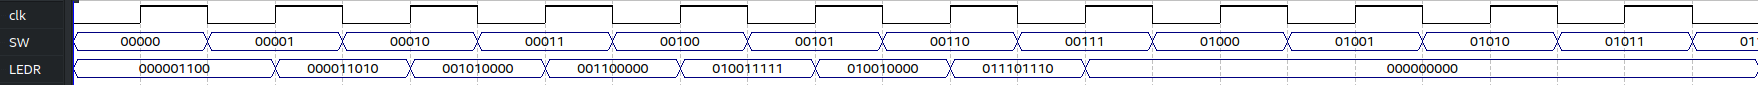
\includegraphics[scale=0.38]{images/Exc3_waveform.png}
\end{figure}

\end{document}